\documentclass[10pt,a4paper]{article}
\usepackage[utf8]{inputenc}
\usepackage[italian]{babel}
\usepackage{amsmath}
\usepackage{amsfonts}
\usepackage{amssymb}
\usepackage{graphicx}
\usepackage{siunitx}
\usepackage[left=2cm,right=2cm,top=2cm,bottom=2cm]{geometry}
\newcommand{\rem}[1]{[\emph{#1}]}
\newcommand{\exn}{\phantom{xxx}}
\usepackage[italian]{babel}
\usepackage[utf8]{inputenc}
\usepackage{siunitx}
\usepackage{graphicx}
\usepackage{xcolor}
\usepackage{amsfonts}
\usepackage{amsmath}
\usepackage{amsthm}
\usepackage{tikz}
\usepackage{pgfplots}
\usepackage{enumitem}
\usepackage{siunitx}
\date{\today}
\usetikzlibrary{shapes.geometric,calc,matrix,arrows,snakes,shapes,patterns}
\title{Esercitazione 11B: Flip-Flop e contatori}
\author{Massimo Bilancioni, Alessandro Foligno, Giuseppe Zanichelli}
\begin{document}	
\maketitle
	
\section{ Flip-Flop D-Latch}
\subsection{Montaggio}
 Si monta il circuito come in Figura \ref{circ}; per attivare a piacimento l'Enable lo si collega con un interruttore a terra in modo tale che quando l'interruttore è aperto, Enable è in alto, quando è chiuso Enable è a terra.
 \begin{figure}[h]
 	\label{circ}
 	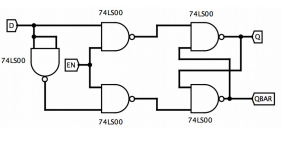
\includegraphics[scale=1]{circuito.png}

 	\caption{schema del circuito realizzato}
 \end{figure}
\subsection{Tempi di ritardo}
Si verifica che quando l'interruttore è aperto ($En=1$), il circuito copia il valore di $D$ su $Q$, nel caso opposto, il valore di $Q$ resta costante. Tenendo il valore di $En$ alto, si manda in ingresso su $D$ un'onda quadra, per misurare il tempo di ritardo. \\Le misure ricavate sono(i segnali osservati sono riportati in Figura \ref{dlatch}):\\ $\Delta t_{salita}\approx40 ns$
\\$\Delta t_{discesa}\approx60 ns$\\
\begin{figure}[h]

	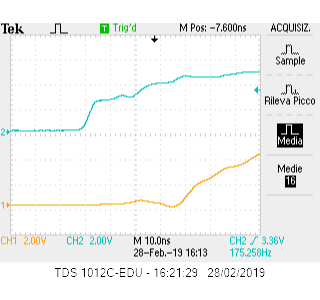
\includegraphics[scale=0.7]{ritardo2.png}
	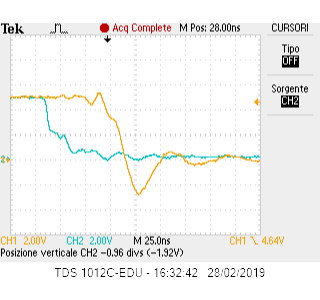
\includegraphics[scale=0.7]{ritardodiscesa2.png}
	\caption{D-Latch con Enable on e in ingresso un'onda quadra: tempo di ritardo in salita e discesa}
		\label{dlatch}
\end{figure} 
La differenza di tempi fra salita e discesa può essere spiegata dando un'occhiata al circuito. Quando $D$ va in alto, il nuovo segnale deve passare attraverso il primo NAND e dare FALSE, dopodichè il NAND successivo restituirà immediatamente TRUE, indipendentemente dal segnale su $\bar{Q}$. Invece, quando $D$ diventa FALSE,il NAND che restituisce $Q$ avrà ad un ingresso TRUE e all'altro $\bar{Q}$, quindi affinchè il segnale su $Q$ sia quello giusto, deve prima arrivare il segnale corretto su $\bar{Q}$ e quindi bisogna passare attraverso altri due NAND, con un ritardo di circa $10 ns$ ciascuno. Questo spiega anche perchè il segnale sull'oscilloscopio(arancione) è così diverso da quello in ingresso (quello blu).

\textcolor{red}{NON SO SE DEVI ANCORA FINIRE IN OGNI CASO AGGIUNGI L'ENABLE LA FIGURA}
\section{ Divisori di frequenza }
Si è montato il circuito in figura come mostrato nell'immagine \textcolor{red}{AGGIUNGERE IMMAGINE}.
Si è verificato il corretto funzionamento del contatore con un impulso a bassa frequenza.

Abbiamo inviato un clock a una frequenza di circa $f\simeq 50 \si{\kilo \hertz}$; nelle immagini che seguono compaiono  rispettivamente $Q0$, $Q1$, $Q2$  (in giallo) sovrapposti al clock (in blu), dalle figure si vede che le frequenze sono effettivamente $1/2$, $1/4$, $1/8$ di $f$. Per $Q3$, segnale di cui non compare l'immagine è stato verificato che la sua frequenza fosse $1/16$ di quella del clock.
\begin{figure}[h]
			\centering
			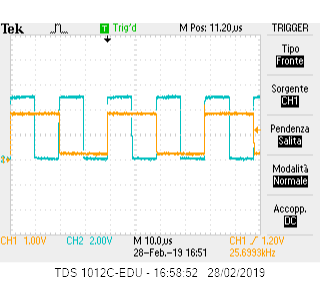
\includegraphics[scale=0.85]{1mezzo}
			\caption{sengale $Q0$ in blu}
			\label{fig:plh}
\end{figure}
\begin{figure}[h]
			\centering
			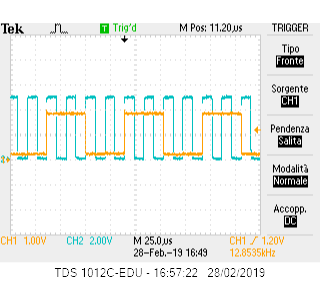
\includegraphics[scale=0.85]{1quarto}
			\caption{sengale $Q1$ in blu}
			\label{fig:plh}
\end{figure}
\begin{figure}[h]
			\centering
			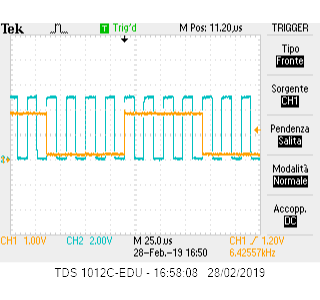
\includegraphics[scale=0.85]{1ottavo}
			\caption{sengale $Q2$ in blu}
			\label{fig:plh}
\end{figure}
Tramite l'oscilloscopio si è poi misurato il ritardo tra la transizione del clock e quella di $Q0$, $Q1$, $Q2$ e $Q3$; in particolare si è misurato l'intervallo temporale che intercorreva da quando la tensione in ingresso passava per il $50\%$ del valore massimo a quando l'uscita passava per  il $50\%$ del valore massimo. Nelle Figure \ref{fig:t1} e \ref{fig:t2} sono mostrati il segnale di clock (in blu) e $Q0$ (in giallo) rispettivamente quando il segnale  $Q0$ passa da alto a basso e da basso ad alto. I ritardi misurati per questa uscita 
sono nel primo caso $t\ped{discesa} = (150 \pm 5)\si{\nano\second}$ e nel secondo  $t\ped{salita} = (30 \pm 5)\si{\nano\second}$.\textcolor{red}{CONTROLLARE COERENZA ERRORI NEI RITARDI PUNTO 2-3}
Per gli altri tre i ritardi sono gli stessi di $Q0$  nei due casi, infatti le quattro uscite sono quasi perfettamente sincrone tra loro; come esempio  di questa sincronia mostriamo  i segnali $Q0$ e $Q1$ nella transizione da alto a basso in Figura \ref{fig:q0q1}.
Sul datasheet è riportato come tempo di propagazione massimo dal clock all'output (una qualsiasi delle $Q$) $t\ped{max} = 15\si{\nano\second}$ sia per la transizione $HL$ che $LH$. La discrepanza può essere dovuta al tempo di salita del generatore (clock) che avviene in un tempo di circa $50 \si{\nano\second}$, questo potrebbe giustificare il risultato ottenuto per $t\ped{salita} $ tuttavia non giustifica l'asimmetria dei due risultati e il valore misurato per $t\ped{discesa}$.
\textcolor{red}{CONFRONTARE TEMPI CON DATASHIIIIIT NON TORNA NULLA!}
\begin{figure}[h]
			\centering
			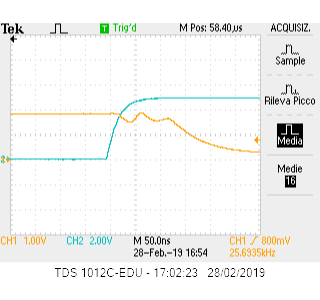
\includegraphics[scale=0.85]{tcounter}
			\caption{ritardo di $Q0$ nel passare da alto a basso}
			\label{fig:t1}
\end{figure}
\begin{figure}[h]
			\centering
			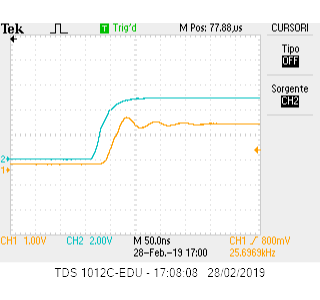
\includegraphics[scale=0.85]{tcounter_1}
			\caption{ritardo di $Q0$ nel passare da basso ad alto}
			\label{fig:t2}
\end{figure}

\begin{figure}[h]
			\centering
			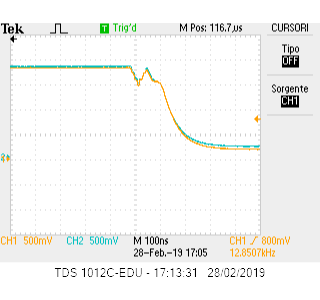
\includegraphics[scale=0.85]{Q0Q1sincroni}
			\caption{quasi perfetta sincronia tra i segnali $Q0$ e $Q1$ quando entrambi diventano bassi}
			\label{fig:q0q1}
\end{figure}

Per resettare il circuito a $10$  abbiamo collegato i segnali $Q1$ e $Q3$ a una porta NAND e l'uscita della porta  al $\overline{\mathrm{CLR}}$ del contatore a $4$-bit di modo che appena entrmabi fossero stati alti il conteggio si sarebbe resettato.
\section{ Shift register con D-Latch}



\end{document}